\documentclass[12pt, oneside, openany]{book}

\usepackage{mathptmx} % Contiene una fuente similar a Times New Roman

\usepackage[spanish, es-tabla]{babel} % Permite escritura en castellano
\usepackage[utf8]{inputenc} % Permite utilizar caracteres UTF8

\usepackage{graphicx} % Para la inclusión de gráficos e imágenes
\graphicspath{ {images/} } % Ruta para buscar las imágenes
\usepackage[a4paper,top=30mm,left=30mm,right=25mm,bottom=25mm,headheight=20mm]{geometry} % Configuración de los margenes de la página

% Paquetes para que funcione el formato.
\usepackage{titlesec}
\usepackage{setspace}
\usepackage{ragged2e}
\usepackage{fancyhdr}
\usepackage{lastpage}
\usepackage{stackengine}
\usepackage{array}
\usepackage[hidelinks]{hyperref}
\usepackage{enumitem}
\usepackage{float}
\usepackage{hypcap}
\usepackage{caption}
\usepackage{fancyvrb}

\usepackage{hyperref} % Paquete para que las referencias funcionen, y permite introducir links
\usepackage{xcolor} % Paquete para trabajar con colores (fondo de celdas, color del texto...)
% Se define un color gris desde su código RGB
\definecolor{gris}{RGB}{220,220,220}

\setcounter{secnumdepth}{3} % Para permitir numerar las sub-subsecciones

% Modifica el nombre de los índices al castellano
\addto\captionsspanish{
  \renewcommand{\contentsname}{Índice de contenido}
  \renewcommand{\listfigurename}{Índice de figuras}
  \renewcommand{\listtablename}{Índice de tablas}
  \renewcommand{\lstlistingname}{Listado}
  \renewcommand{\lstlistlistingname}{Índice de listados}
}

% Formateo de los nombres de los apartados:
\titleformat{\chapter}[block]
{\normalfont\Huge\bfseries\singlespacing}{\thechapter.}{1em}{\Huge}
\titlespacing*{\chapter}{0pt}{-62pt}{0pt}

\titleformat{\section}[block]
{\normalfont\Large\bfseries}{\thesection.}{4pt}{\Large}
\titlespacing*{\section}{0pt}{\baselineskip}{0pt}

\titleformat{\subsection}[block]
{\normalfont\large\bfseries}{\thesubsection.}{4pt}{\normalsize\large}
\titlespacing*{\subsection}{0pt}{0pt}{0pt}

\titleformat{\subsubsection}[block]
{\normalfont\normalsize\bfseries}{\thesubsubsection.}{4pt}{\normalsize}
\titlespacing*{\subsubsection}{0pt}{0pt}{0pt}

\def\tablename{Tabla}

%% Variables para portada y cabeceras
%% Cambiar los valores para cada documento!!!
\def\title{Explotación, integración y visualización de múltiples fuentes de datos mediante un Data Lake}
\def\shortTitle{ETL de datos heterogéneos mediante un Data Lake}
\def\subject{Lenguajes y Sistemas Informáticos}
\def\author{Mier Montoto, Juan Francisco}
\def\date{julio 2024}
\def\org{Escuela Politécnica de Ingeniería de Gijón}
\def\area{Grado en Ingeniería Informática en Tecnologías de la Información}
\def\tutorOne{D. Augusto Alonso, Cristian}
\def\tutorTwo{D. Morán Barbón, Jesús}
\def\tutorThree{D. Vázquez Faes, Eduardo}
\def\tfgId{???}

\def\ORG{\expandafter\MakeUppercase\expandafter{\org}}
\def\AREA{\expandafter\MakeUppercase\expandafter{\area}}
\def\SUBJECT{\expandafter\MakeUppercase\expandafter{\subject}}


\captionsetup{justification=centering}
\setlength{\headheight}{65pt}

\fancyhf{}
\fancyhead[L]{
\includegraphics[height=16mm]{style/square.png}
  \hspace{1em} \Longstack[l] {
    \textbf{\SUBJECT} \newline
    \textbf{\shortTitle}}
  \newline \leftmark{}
}
\fancyhead[R]{\bfseries{Hoja \hyperlink{toc}{\thepage}~de~\pageref{LastPage}}}
\fancyfoot[C]{\author}
\renewcommand{\headrulewidth}{0pt} % default is 0pt
\renewcommand{\footrulewidth}{0.4pt} % default is 0

\fancypagestyle{plain}{%
  \fancyhf{}
  \fancyhead[L]{
\includegraphics[height=16mm]{style/square.png}
    \hspace{1em} \Longstack[l]{
      \textbf{\SUBJECT} \newline
      \textbf{\shortTitle}}}
  \fancyhead[R]{\bfseries{Hoja \hyperlink{toc}{\thepage}~de~\pageref{LastPage}}}
  \fancyfoot[C]{\author}
  \renewcommand{\headrulewidth}{0pt} % default is 0pt
  \renewcommand{\footrulewidth}{0.4pt} % default is 0pt
}

\newcommand*{\fullref}[1]{\textit{\hyperref[{#1}]{\ref*{#1} \nameref*{#1}}}}

\pagestyle{fancy}

\restylefloat{table}
\definecolor{backcolour}{rgb}{0.95,0.95,0.92}
\definecolor{darkgreen}{rgb}{0.0, 0.5, 0.0}

\lstdefinestyle{default}{
  basicstyle=\ttfamily\footnotesize,
  breakatwhitespace=false,
  breaklines=true,
  captionpos=b,
  keepspaces=true,
  numbers=left,
  numbersep=5pt,
  numberstyle=\tiny\color{black},
  showspaces=false,
  showstringspaces=false,
  showtabs=false,
  tabsize=2,
  backgroundcolor=\color{backcolour},
  postbreak=\mbox{\textcolor{red}{$\hookrightarrow$}\space},
}

\lstset{style=default}

\lstdefinestyle{yaml}{
  basicstyle=\ttfamily\footnotesize\color{darkgreen}\bfseries,
  rulecolor=\color{black},
  string=[s]{'}{'},
  stringstyle=\color{darkgreen},
  comment=[l]{:},
  commentstyle=\color{blue},
  morecomment=[l]{-},
  numbers=left,
  numbersep=5pt,
  numberstyle=\tiny\color{black},
  backgroundcolor=\color{backcolour},
  breaklines=true,
  captionpos=b,
  keepspaces=true,
  showspaces=false,
  showstringspaces=false,
  showtabs=false,
  tabsize=2,
  breakatwhitespace=true,
  postbreak=\mbox{\textcolor{red}{$\hookrightarrow$}\space},
}



\begin{document}

\rmfamily % Fuente tipo Romana

% Portada de la memoria
\begin{titlepage}
    \centering
    \bfseries {
        \null{}
        \vspace{0cm}
        \begin{table}[h]
            \centering
            \begin{tabular}{m{10cm} m{1cm} m{3cm}}
                \vspace{0.2cm}
                
\includegraphics[width=86mm]{style/full.png} &  & \vspace{1.52mm} 
\includegraphics[width=23mm]{style/square.png} \\
            \end{tabular}
        \end{table}

        \vspace{3\baselineskip}

        \Large{\ORG{} \\ \vspace{3\baselineskip}}
        \large {
            \AREA{} \\ \vspace{3\baselineskip}
            \subject{} \\ \vspace{2\baselineskip}

            TRABAJO FIN DE GRADO/MÁSTER Nº \tfgId{} \vspace{\baselineskip} \\
            \title{} \\ \vspace{1\baselineskip}

            \author{} \\ \vspace{1\baselineskip}
            TUTORES:\\
            \tutorOne{} \\
            \tutorTwo{} \\
            \tutorThree{} \\ \vspace{\baselineskip}

            \vspace{2\baselineskip}
            FECHA:\@ \date{}
        }
    }
\end{titlepage}


% Índice de contenido
\addcontentsline{toc}{chapter}{Índice de contenido} % Añade la referencia al índice de contenido
\hypertarget{toc}{}
\tableofcontents
\newpage

% Índice de figuras
\addcontentsline{toc}{chapter}{Índice de figuras}  % Añade la referencia al índice de contenido
\hypertarget{lof}{}
\listoffigures

\justify{} % Texto justificado
\setlength{\parskip}{\baselineskip} % Separación entre párrafos de 1 linea
\onehalfspacing{}

%% El contenido de la memoria, dividido en capítulos:
\chapter{Introducción}\label{chap:intro}
En este capítulo se presenta una introducción al trabajo de desarrollo de software realizado,
proporcionando un contexto general y estableciendo el escenario para los capítulos siguientes.
Se discutirán los antecedentes y la motivación detrás de este trabajo, la finalidad del proyecto,
y se proporcionará una breve descripción de la empresa en la que se ha desarrollado este trabajo.
Este capítulo tiene como objetivo proporcionar una visión general del proyecto y establecer las
bases para los capítulos detallados que siguen.

\section{Antecedentes}\label{sec:antecedentes}
Hoy en día, nos encontramos en una era donde la generación y almacenamiento de datos crece
exponencialmente\footnote{\url{https://www.statista.com/statistics/871513/worldwide-data-created/}},
un hecho que se ve reflejado en el ámbito empresarial. La diversidad de fuentes y formatos de
estos datos introduce una complejidad significativa en su manejo, conocida como \textit{heterogeneidad}
\footnote{\url{https://www.sciencedirect.com/topics/computer-science/data-heterogeneity}}, siendo las
bases de datos, archivos de registros y APIs las fuentes más habituales.

El término \textit{big data} describe este fenómeno de acumulación masiva de datos, cuya magnitud y
complejidad sobrepasan las capacidades de los métodos de procesamiento convencionales. El \textit{big data}
por tres características principales: volumen, variedad y velocidad - su adecuada gestión y análisis
pueden otorgar ventajas competitivas significativas a las empresas, tales como el descubrimiento de
patrones ocultos, identificación de nuevas oportunidades de mercado y optimización de procesos de toma
de decisiones.

Uno de los procesos que permite la extracción de esta información es la pirámide DIKW, \cite{enwiki:1211227190}
es un modelo que describe la relación entre los datos, la información, el conocimiento y la sabiduría.
Según este modelo, los datos son la materia prima de la información, que a su vez es la materia prima
del conocimiento, que a su vez es la materia prima de la sabiduría. Una organización sin los procesos
adecuados para la gestión y análisis de estos datos, se enfrenta a importantes desafíos, como la dificultad
para identificar patrones y tendencias, la toma de decisiones incorrectas y la pérdida de oportunidades de
negocio. Por otro lado, una organización que logre extraer información valiosa de sus datos, podrá mejorar su
eficiencia, aumentar su competitividad y adaptarse mejor a un entorno empresarial en constante cambio.

La evolución tecnológica ha propiciado el desarrollo de innovadoras herramientas y metodologías
diseñadas para enfrentar estos desafíos. Entre ellas, los \textit{data lakes} (o \emph{lagos de
información}) se destacan por su capacidad para consolidar vastos volúmenes de datos heterogéneos,
facilitando su posterior análisis y aprovechamiento de manera más efectiva.

Sin embargo, a pesar de que existen herramientas de almacenamiento, el proceso de integración,
visualización y análisis de estos datos es una tarea desafiante, ya que requiere de una gran
cantidad de recursos y de un tiempo de desarrollo considerable del que, normalmente, no se dispone
en el ámbito empresarial.

Con la ingesta masiva de datos, se presentan nuevos problemas a la hora de analizar y obtener
información de ellos:

\begin{itemize}
	\item Sin la necesaria automatización y correcta aplicación de los procesos ETL,
		al tratarse de un crecimiento exponencial de los datos y, por lo tanto, de la fuerza
		de trabajo necesaria para manejarla, los resultados del análisis pueden ser incorrectos,
		lo que deriva en errores y decisiones de negocio equivocadas que impactan negativamente
		en la empresa.
	\item La heterogeneidad de los datos, tanto en formato como en origen, dificulta su
		consolidación y análisis.
	\item La masificación de información impide el análisis manual de los mismos, requiriendo resúmenes
		estadísticos o representaciones gráficas como \textit{dashboards} para su correcta interpretación.
		La visualización de datos es una técnica que permite representar la información de manera visual,
		para facilitar su análisis y comprensión. La visualización de datos es una parte importante del
		proceso de análisis de datos, ya que permite identificar patrones, tendencias y anomalías en los
		datos de forma más rápida y sencilla.
\end{itemize}

\newpage{}
\section{Motivación}\label{sec:motivacion}
Okticket, como el resto de empresas, se enfrenta a la necesidad de gestionar y analizar grandes
volúmenes de datos, provenientes de múltiples fuentes y en diferentes formatos. La correcta gestión
y análisis de estos datos es fundamental para la toma de decisiones y para la mejora de los procesos
internos de la empresa.

En la actualidad, la empresa dispone de una gran cantidad de datos que se encuentran en
diferentes formatos y en diferentes ubicaciones, lo que dificulta su análisis y explotación.
Por otra parte, se depende de la consulta manual o de servicios de terceros para poder analizar
estos datos, lo que supone un coste adicional.

El proyecto surge de la necesidad de la empresa de extraer información y conocimiento de las
múltiples y heterogéneas fuentes de datos de las que se disponen, tanto internas (e.g.~bases de
datos, archivos de registros, APIs, entre otros), como externas (e.g. APIs o datos de webs de
terceros, datos de fuentes públicas\ldots).

Además del uso interno, la empresa también quiere ofrecer a sus clientes la posibilidad de
consultar estos datos de forma visual y sencilla, para que puedan analizarlos y explotarlos de
forma autónoma, lo que supondría un valor añadido para los mismos.

\newpage{}
\section{La empresa}\label{sec:empresa}
Okticket es una startup nacida en Gijón en 2017 cuyo producto principal es un servicio software que escanea
automáticamente de tickets y notas de gastos lo que permite reducir los costes y el tiempo que invierten
las empresas en contabilizar y manejar los gastos de viaje de los profesionales.

La empresa tienen su suede principal en el Parque Tecnológico de Gijón, aunque cuenta con un número
de sedes creciente en varios países, como Francia, Portugal o, más recientemente, México. En esta
oficina principal se encuentran los departamentos de ventas y marketing, así como el equipo de
desarrollo y soporte.

Okticket es una de las empresas que más crecen tanto del sector como del propio Parque
Tecnológico. Debido a este rápido crecimiento, el equipo está en constante desarrollo y
cambio, tanto aquí en España como en el resto de sedes. Este crecimiento se refleja
en la recepción de un gran número de galardones y reconocimientos.
\footnote{\href{https://www.linkedin.com/posts/okticket_okticket-en-el-especial-startups-de-forbes-activity-7140622980618903552-UGWK}{Okticket en el especial startups 2023 de Forbes (LinkedIn)}}
\footnote{\href{https://www.elcomercio.es/economia/arcelor-okticket-premios-20230222002438-ntvo.html}{Arcelor y Okticket, premios nacional de Ingeniería Informática (EL COMERCIO)}}
\footnote{\href{https://www.okticket.es/blog/empresa-pyme-innovadora}{Okticket recibe el sello Pyme Innovadora (okticket.es)}}
\footnote{\href{https://www.okticket.es/blog/okticket-empresa-emergente-certificada}{Okticket, empresa emergente certificada (okticket.es)}}

La parte principal del negocio es el núcleo del software como servicio (Software as a
Service en inglés, en adelante \textit{SaaS}), es decir, la aplicación completa tanto
para administradores como para empleados. Este SaaS se oferta a empresas de cualquier
tamaño, cuyo precio final varía en función del número de usuarios, las características
e integraciones que requiera la empresa cliente y el soporte que se ofrezca.

Recientemente se han añadido nuevas propuestas a la cartera de servicios ofertada por
Okticket, como la OKTCard {-} una tarjeta inteligente que gestiona automáticamente los gastos,
así como la inclusión de nuevos ``módulos'' de gestión de gastos y viajes.

Debido a todo este crecimiento, la empresa maneja una gran cantidad de datos importantes que se
encuentran en diferentes formatos y en diferentes ubicaciones, lo que dificulta su análisis y
explotación. Por otra parte, se depende de la consulta manual o de servicios de terceros para
poder analizar estos datos, lo que supone un coste adicional.

\section{Objetivos}\label{sec:objetivos}
El objetivo del proyecto es el desarrollo y despliegue de una infraestructura de datos que permita
la integración, almacenamiento y análisis de grandes volúmenes de datos, provenientes de múltiples
fuentes y en diferentes formatos. La infraestructura de datos debe ser escalable, flexible y
robusta, para poder adaptarse a las necesidades cambiantes de la empresa.

La infraestructura de datos debe permitir la integración de datos de múltiples fuentes, tanto
internas como externas, y en diferentes formatos, como bases de datos, archivos de registros, APIs,
entre otros. La integración de datos debe ser automática y programable, para poder automatizar el
proceso de ingestión de datos y reducir el tiempo y los costes asociados.

Pese a que el entregable principal de este proyecto es la creación de una infraestructura, se
esperan también otros entregables en forma de herramientas de software, como \textit{scripts},
que faciliten la integración y análisis de los datos, así como la visualización de los mismos.

\chapter{Fundamento teórico}\label{chap:teo}
En este capítulo se presentan los conceptos y términos fundamentales que se utilizan en el
proyecto, para proporcionar una base teórica sobre la que se desarrolla el trabajo. Se discuten
los conceptos de \textit{data lake}, \textit{procesos ETL} y \textit{dashboards}, que son
fundamentales para el desarrollo del proyecto.

\section{Paradigmas de almacenamiento de datos}\label{sec:paradigmas}
En el ámbito de la gestión de datos, existen diferentes paradigmas de almacenamiento de datos
que se utilizan para almacenar y analizar grandes cantidades de información. Los tres paradigmas
a considerar para este proyecto son los \textit{data warehouses}, los \textit{data lakes} y los
\textit{data lakehouses}.

\subsection{Data warehouse}\label{sec:warehouse}
Un \textit{data warehouse}\footnote{\url{https://aws.amazon.com/es/data-warehouse/}},
también conocido en español como almacén de datos, es una base de datos que se utiliza para
almacenar y analizar grandes cantidades de datos de manera eficiente. Los almacenes de datos
proporcionan acceso rápido y compatible con plataformas de consultas (como SQL) a grandes
cantidades de datos, lo que permite a los analistas y a los científicos de datos realizar
análisis complejos sobre los datos almacenados.

Todos los datos almacenados en un \textit{data warehouse} se encuentran en un formato común,
para lo que se aplican procesos ETL (extracción, transformación y carga) que transforman los
datos de diferentes fuentes en un formato común. Esto significa que la información se
encuentra en un formato o esquema optimizado y específico, lo que facilita su manipulación y
análisis pero limita la flexibilidad al acceso de los datos y genera costes adicionales en
el caso de tener que modificar o transferir los mismos para su uso.


\subsection{Data lake}\label{sec:lake}
Los \textit{data lakes}\footnote{\url{https://aws.amazon.com/es/what-is/data-lake/}}
son almacenes de datos que guardan grandes cantidades de datos de manera no
estructurada~\cite{mier2023dashboards}. En el ámbito de una empresa, un \textit{data lake}
contiene datos de diferentes fuentes de valor no considerado hasta su análisis, de manera
que su explotación posterior y su análisis no depende de una estructuración y transformación
compleja, reduciendo los costes de los procesos ETL derivados, una flujo de tareas que se
aplican sobre la información para ingestarla. Esto no quiere decir que no se apliquen estos
procesos a los datos, sino que se aplican de manera más flexible y básica que en otras
estructuras de almacenamiento de datos con esquemas predefinidos, como los
\textit{data warehouses}.~\cite{pwint2018data}

A diferencia de los \textit{data warehouses}, los \textit{data lakes} no tienen un
esquema definido, lo que permite almacenar datos \textit{heterogéneos}. Esto permite
almacenar grandes cantidades de información sin tener que definir un esquema de antemano,
lo que puede ser útil en aquellos casos en los que no se conoce la estructura de los
datos que se van a almacenar.

Estas características de los \textit{data lakes} hacen que sean más atractivos en el sector
empresarial de cara al análisis de información, en contraste con las estructuras planteadas
normalmente en el campo de la investigación académica.

Para consultar esta gran cantidad de datos almacenados, se suelen utilizar técnicas de
visualización de datos, como los \textit{dashboards}, herramientas de visualización que
permiten observar los datos de manera sencilla y eficiente.

\subsection{Data lakehouse}\label{sec:lakehouse}
Los \textit{data lakehouses} son una combinación funcional de los dos paradigmas vistos
anteriormente, los \textit{data lakes} y los \textit{data warehouses}. Los \textit{data
lakehouses} permiten almacenar datos tanto de manera estructurada como no estructurada,
lo que facilita aprovechar la información al contar con una única estructura de bajo coste
que ofrece a los usuarios que lo necesiten explorar y analizar los datos según sus necesidades.

Puesto que en este proyecto se plantea el uso de datos tanto estructurados como no estructurados,
y no siempre será de interés aplicar procesos de transformación a toda la información obtenida,
los \textit{data lakehouse} se presentan como una solución eficiente y flexible para el almacenamiento
y análisis de los datos.

\newpage{}
\section{Procesos ETL}\label{sec:etl}
Los procesos ETL~\cite{mier2023dashboards} son procesos que combinan datos de múltiples
fuentes en un único destino, transformando los datos en un formato común. Estos procesos
se utilizan para extraer datos de diferentes fuentes, transformarlos en un formato común
y cargarlos en un destino común, como puede ser un \textit{data lake}.

% \subsection{Características}
Los procesos ETL, fundamentales en el ámbito de la gestión de datos, presentan atributos
distintivos que facilitan la integración eficaz de información procedente de diversas fuentes:

\begin{itemize}
	\item \textbf{Adaptabilidad:} los procesos ETL deben de adaptarse a la estructura de los
		datos de la fuente de origen, ya que dichas fuentes pueden tener diferentes estructuras
		y tener tipos de datos diferentes (la característica de \textit{heterogeneidad} de los
		datos que ya se ha mencionado).
	\item \textbf{Escalabilidad:} otra de las características clave de los procesos ETL es que sean
		escalables, ya que los datos que se muestran en los dashboards suelen ser datos que se generan
		de manera continua, y por lo tanto los procesos ETL deben ser capaces de procesar grandes
		cantidades de datos de manera eficiente. En ocasiones, los procesos ETL se pueden realizar en
		\textit{streaming}, lo que significa que los datos se procesan en tiempo real a medida que se
		generan.
\end{itemize}

\newpage{}
\subsection{Funcionamiento}
Los procesos ETL se dividen en tres fases principales: \textit{extracción}, \textit{transformación}
y \textit{carga}, como se muestra en el sigiuente diagrama:

\begin{minipage}{\linewidth}
	\centering
	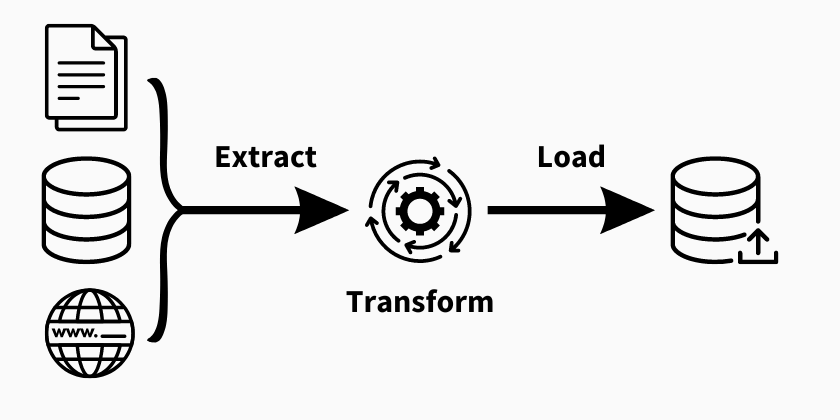
\includegraphics[width=0.8\textwidth]{etl.png}
	\captionof{figure}{Fases de un proceso ETL (trabajo propio)}
\end{minipage}

Al comienzo del proceso, se tienen datos presúntamente heterogéneos que no se pueden analizar de
manera eficiente. Tras aplicar todos los pasos de las fases anteriores, se obtiene un conjunto de
datos homogéneos y listos para ser analizados en el destino indicado (en el caso de este proyecto,
un \emph{data lake}).

\paragraph{Extracción (1)}
En este proceso se extraen los datos de las fuentes de datos, que pueden ser bases de datos, logs,
APIs, etc. En este paso, se pueden aplicar filtros para extraer solo los datos que se necesiten, y
se pueden extraer datos de múltiples fuentes \emph{heterogéneas}.

En algunos casos, los datos se pueden extraer de manera incremental, es decir, solo se extraen los
datos que han cambiado desde la última extracción. Esto puede ser útil para reducir el tiempo de
procesamiento y el volumen de datos que se almacenan.

En otros casos, los datos se pueden extraer de manera continua, es decir, se extraen los datos en
tiempo real según se van generando. Esto puede ser útil para procesar datos que se generan en tiempo
real, como logs o datos de sensores.

\newpage{}
\paragraph{Transformación (2)}
En este proceso se transforman los datos extraídos en la fase anterior, normalmente aplicándoles
un proceso de limpieza y transformación a un formato común. En este paso, se pueden aplicar
diferentes operaciones a los datos, como la limpieza, la agregación, la normalización, la conversión
de formatos, etc.

Una transformación especialmente importante que se suele reaizar durante este proceso es la limpieza,
revisión y corrección de los datos extraídos, para asegurar que se almacena información correcta y
consistentes. Durante esta fase se contemplan operaciones más complejas, como pueden ser la agregación
de datos, la conversión de formatos, la normalización de datos, el cifrado, etc.

Estos procesos de transformación son vitales cuando el sistema maneja una gran cantidad de datos heterogéneos
de múltiples fuentes de manera simultánea, como puede ser el caso de un \textit{data lake} o un \textit{data
warehouse}. En el caso del primero, no es necesaria la transformación de los datos a un formato común, pero si
otros procesos clave como la limpieza y la normalización de los datos, entre otros.

\paragraph{Carga (3)}
En este proceso se cargan los datos transformados en el destino final. Frecuentemente, los datos se
almacenan en una data warehouse o data lake para su posterior análisis.

La frecuencia del proceso de carga depende de la naturaleza de los datos y de las necesidades del
negocio, como ya se ha descrito en el proceso de extracción.

Tras completar este proceso, los datos están listos para ser analizados y visualizados desde las arquitecturas
de datos que almacenen la información.

\newpage{}
\subsection{Alternativas}
Aunque lo más común es el flujo anteriormente explicado de \textit{extracción}, \textit{transformación} y
\textit{carga}, existen algunos flujos y procesos alternativos que evitan algunos de estos pasos, normalmente
en casos específicos que se beneficien del cambio:

\begin{itemize}
	\item \textbf{Virtualización de datos:} capa virtual de abstracción que permite acceder a los datos de las
		fuentes sin necesidad de extraerlos. Esto permite ahorrar espacio de almacenamiento y tiempo de procesamiento,
		pero suele ser menos eficiente en términos de rendimiento y no es compatible con todas las arquitecturas de
		datos.

		\begin{minipage}{\linewidth}
			\centering
			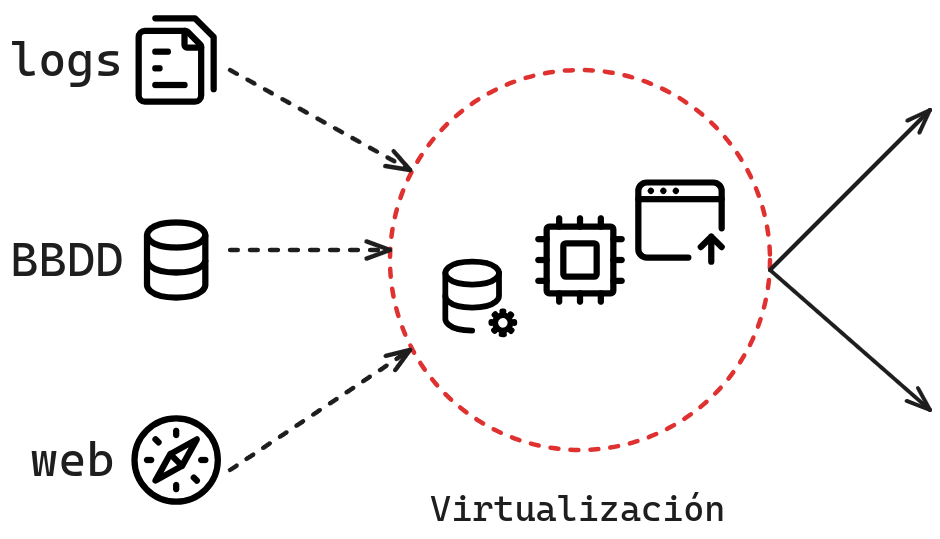
\includegraphics[width=0.65\textwidth]{virt.png}
			\captionof{figure}{Ejemplo de flujo con virtualización (trabajo propio)}
		\end{minipage}
	\item \textbf{Proceso \textit{ELT}\footnote{\url{https://www.ibm.com/topics/elt}}:} en lugar de transformar
		los datos antes de cargarlos en el destino, se cargan los datos en bruto y se transforman en el destino.
		Funciona bien para grandes conjuntos de datos sin estructura que requieran una carga (o recarga) contínua,
		aunque, al igual que la virtualización, puede ser menos eficiente o incompatible con algunas arquitecturas
		de datos, como los \textit{data warehouses}.

		\begin{minipage}{\linewidth}
			\centering
			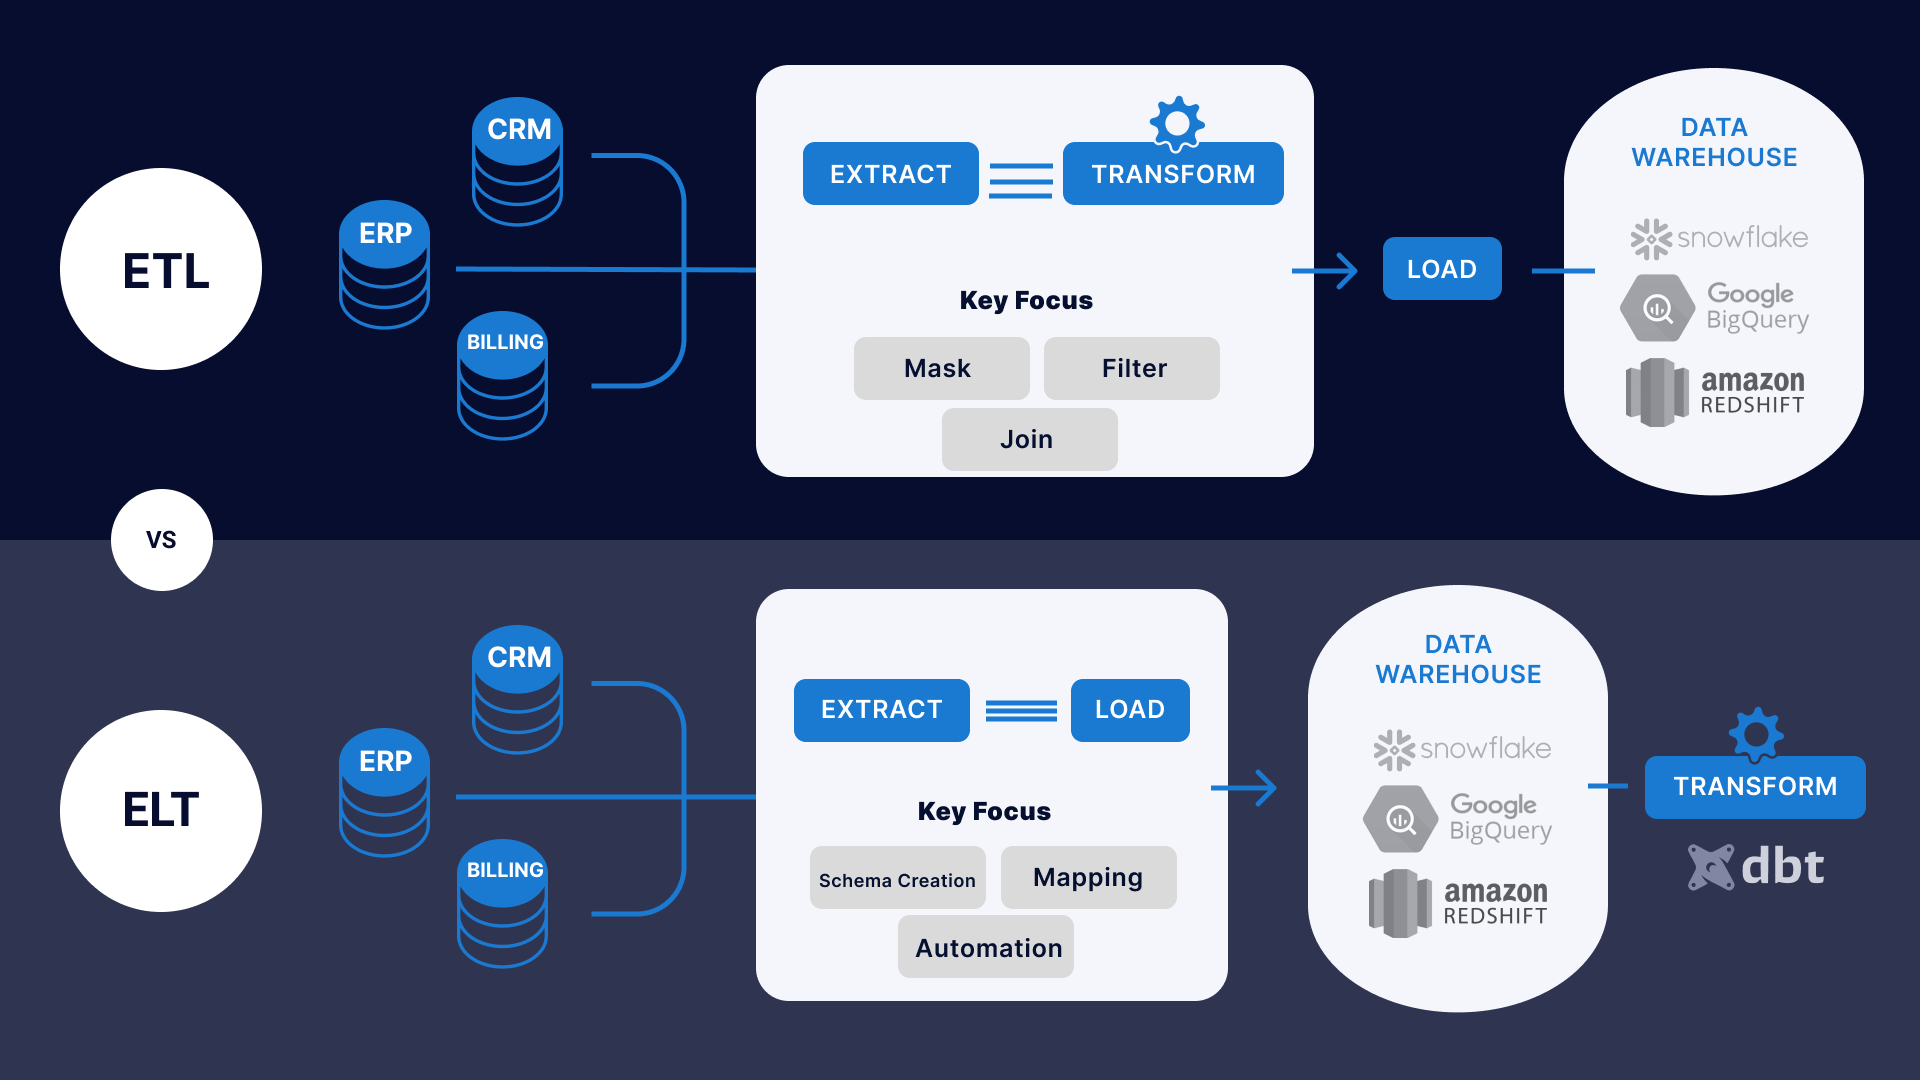
\includegraphics[width=0.75\textwidth]{elt.png}
			\captionof{figure}{Diagrama de flujo de un proceso \textit{ELT} (trabajo propio)}
		\end{minipage}
\end{itemize}


\newpage{}
\section{Dashboards}\label{sec:dashboards}
\paragraph{Definición}
La palabra \textit{dashboard}, que traducido de manera literal significa \textit{cuadro de mandos},
es un término que se utiliza para referirse a cualquier interfaz gráfica que muestre información
relevante de manera visual sobre un proceso o negocio. Aunque el término se utiliza en
muchos ámbitos: indicadores comerciales, de producción, de marketing, de calidad, de recursos
humanos\ldots, en este proyecto se utilizará en el ámbito de la monitorización de sistemas y
procesos de negocio.

En el ámbito de deste proyecto, los dashboards reflejan en tiempo real el rendimiento de
actividades o procesos de negocio, y se utilizan para tomar decisiones informadas sobre los
mismos. En el caso de una empresa, un dashboard puede mostrar desde el rendimiento de la
plataforma en tiempo real hasta un reflejo del de las ventas, y permitir a los directivos tomar
decisiones informadas sobre el futuro de la empresa.

\paragraph{Características}
Los dashboards cuentan con una serie de características que los hacen útiles para la toma de
decisiones:~\cite{mier2023dashboards}

\begin{itemize}
	\item \textbf{Visualización de datos:} es la característica fundamental de cualquier
		cuadro de mandos, y aquella que determina su utilidad. La visualización de datos
		es la ciencia de presentar los datos de manera que se pueda extraer información útil
		y realizar decisiones informadas sobre ellos. Un buen dashboard cuenta con gráficas,
		tablas, indicadores, etc. que permiten al usuario entender la información que se
		está presentando con un conocimiento técnico mínimo.
	\item \textbf{Interactividad y personalización:} un dashboard debe permitir al usuario
		interactuar con los datos (filtrarlos, ordenarlos, profundizar en ellos...) y ajustar
		la información que se muestra a cada proceso o negocio que se esté evaluando.
		Esta capacidad asegura que el dashboard se adapte tanto a las necesidades actuales
		como a las evoluciones futuras de lo que se esté analizando.
	\item \textbf{Accesibilidad y portabilidad:} un dashboard debe ser accesible desde una
		variedad de situaciones y dispositivos, manteniendo su funcionalidad y forma. Aunque
		normalmente los dashboards se analizan en pantallas grandes, es importante que también
		se puedan consultar en otras circunstancias, como dispositivos móviles.
\end{itemize}

\newpage{}
\subsection{Dashboards planteados}
Para el sistema que se describe, se plantean dos tipos de dashboards diferentes:

\begin{itemize}
	\item \textbf{Dashboards internos}: que reflejan el rendimiento de la plataforma en tiempo real.
	\item \textbf{Dashboards externos}: que reflejan el rendimiento de las ventas y permiten a los
	      clientes tomar decisiones informadas sobre su negocio.
\end{itemize}

Hay que destacar que los dashboards externos son diferentes a los dashboards de monitorización, tanto
en el contenido que presentan como en la manera de acceder a ellos: mientras que los dashboards de
monitorización serán de uso interno exclusivo, los dashboards externos deben estar disponibles para
los clientes de las empresas que los contraten.

% mover esta sección a la valoración de alternativas cuando se tenga
% \section{Componentes del sistema}\label{sec:componentes}
% En el \textit{stack} tecnológico escogido para el proyecto se manejan
% diferentes términos y conceptos que son necesarios desarrollar para
% entender el funcionamiento del sistema.

% \subsection{Tópico}\label{subsec:topico}
% Un tópico es una categoría a la que se envían los mensajes a la que los consumidores están
% \textit{suscritos}. Los consumidores pueden estar suscritos a uno o varios tópicos, y los
% productores pueden enviar mensajes a uno o varios tópicos. Los tópicos son la unidad básica
% de organización de los mensajes en cualquier sistema de mensajería de publicación/suscripción.

% \subsection{Productor}\label{subsec:productor}
% El productor es el componente responsable de crear y enviar mensajes al cluster de Kafka.
% Está separado del resto de los componentes y produce mensajes de manera asíncrona y rápida.

% \subsection{Consumidor}\label{subsec:consumidor}
% El consumidor es el componente responsable de leer los mensajes producidos por el productor.
% Está suscrito a un \nameref{subsec:topico} a través del broker y consume los mensajes.

% \subsection{Broker}\label{subsec:broker}
% El broker es el componente responsable de recibir los mensajes producidos por el productor y
% enviarlos a los consumidores. Es el intermediario entre los productores y los consumidores.

% \subsection{Zookeeper}\label{subsec:zookeeper}
% Zookeeper es un servicio de coordinación distribuida que se utiliza para gestionar y coordinar
% los brokers de Kafka. Se encarga de mantener la información de los brokers y de los tópicos.

\chapter{Planificación del proyecto}\label{chap:planif}
La planificación de un proyecto es fundamental para su correcto funcionamiento y desarrollo,
dentro de los plazos y costes establecidos. Se presenta un primer apartado de metodología, un
segundo apartado con la planificación inicial para posteriomente inferir en base a esta el
presupuesto inicial


\section{Metodología}\label{sec:metodología}
En este capítulo se aborda la metodología adoptada para el desarrollo del proyecto, fundamentada
en principios ágiles y enfocada en la entrega continua de valor. La elección de \textit{Scrum},
una metodología que permite elaborar productos software de manera incremental, revisando el
producto continuamente y adaptándolo a las necesidades del cliente, como marco de trabajo subraya
nuestro compromiso con la adaptabilidad y la mejora continua del producto.

La estructura de este capítulo se organiza en torno a la descripción detallada de la metodología
\textit{Scrum}, la visualización de la planificación y las estrategias de comunicación adoptadas.
A través de esta metodología, buscamos optimizar los recursos disponibles, ajustarnos a los plazos
establecidos y garantizar la calidad del producto final.

La implementación de \textit{Scrum} se complementa con herramientas de visualización y gestión de
proyectos, como los tableros \textit{Kanban}, que facilitan la organización y seguimiento de
las tareas. Además, se pone especial énfasis en la comunicación efectiva dentro del equipo de
desarrollo y con los stakeholders, asegurando así una alineación constante con los objetivos del
proyecto. Existen otras variantes de los tableros \textit{Kanban} que se pueden utilizar para
visualizar el progreso de las tareas, pero en este proyecto se ha elegido esta alternativa para
facilitar la visualización de las tareas y su estado.

Este enfoque metodológico no solo refleja la planificación y ejecución del proyecto, sino que
también establece las bases para una gestión eficaz, adaptativa y orientada a resultados.

\subsection{Scrum}\label{subsec:scrum}
Para la planificación del proyecto se ha escogido \textit{Scrum}, una metodología ``ágil'' que se
basa en la realización de iteraciones cortas y en la adaptación a los cambios. La metodología
\textit{Scrum} se estructura en \textit{sprints} (iteraciones cortas de una duración fija),
en las que se llevan a cabo una serie de tareas que se han planificado previamente.

El primer paso de la metodología \textit{Scrum} es la creación de un \textit{product backlog},
una lista ordenada de las tareas a realizar durante el desarrollo del producto, a partir de los
requisitos del sistema, que a su vez son una versión refinada de los requisitos iniciales del
proyecto. A partir de este \textit{product backlog} se planifican las tareas que se llevarán
a cabo en cada \textit{sprint}, de manera que sea posible cumplir con los objetivos del proyecto
en el tiempo establecido.

A diferencia de metodologías tradicionales o \emph{en cascada}, \textit{Scrum} permite la adaptación
a los cambios y la mejora continua del producto, ya que se revisa y se adapta en cada \textit{sprint}
según las necesidades del cliente y del equipo de desarrollo. Por otro lado, \textit{Scrum} se
diferencia de otras metodologías ágiles como \textit{XP} en que no se centra tanto en las
prácticas de desarrollo, sino en la gestión del proyecto y en la entrega de valor al cliente.

\begin{minipage}{\linewidth}
	\centering
	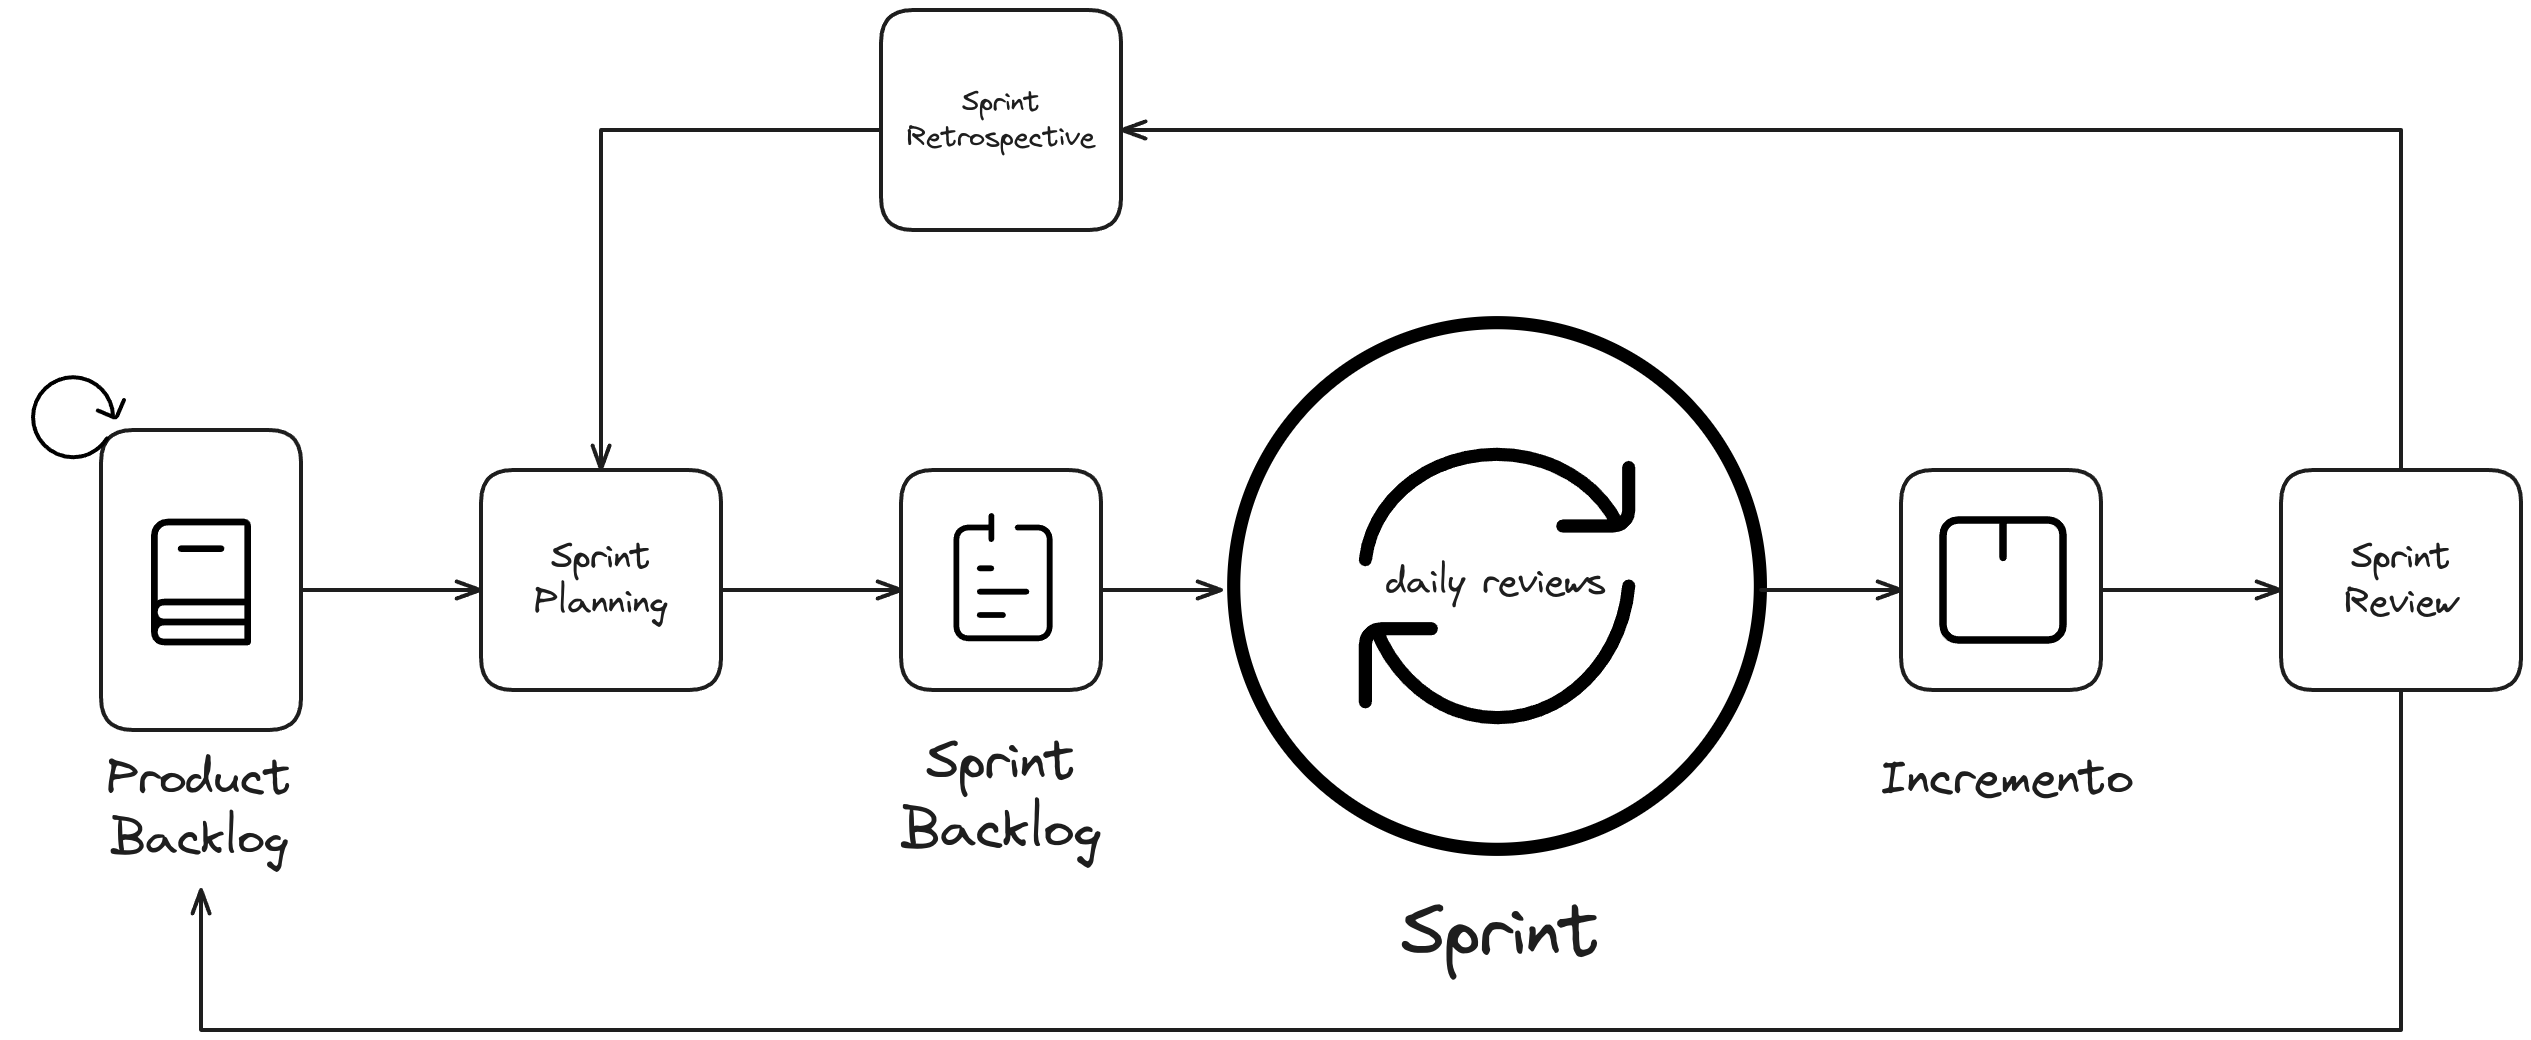
\includegraphics[width=0.85\textwidth]{scrum.png}
	\captionof{figure}{Diagrama de la metodología \textit{Scrum}}
\end{minipage}

\paragraph{Roles}
En \textit{Scrum} se distinguen tres roles principales:

\begin{itemize}
	\item \textbf{Product Owner}: es la persona responsable de definir los requisitos del producto
		y de priorizar las tareas del \textit{product backlog}. Es el enlace entre el equipo de
		desarrollo y el cliente, y es el responsable de garantizar que el producto cumple con las
		expectativas del cliente.
	\item \textbf{Scrum Master}: es la persona responsable de garantizar que el equipo de desarrollo
		sigue la metodología \textit{Scrum} y de eliminar los obstáculos que puedan surgir durante
		el desarrollo del proyecto. El \textit{Scrum Master} es el encargado de organizar las
		reuniones diarias y de asegurar que el equipo de desarrollo cumple con los plazos y los
		objetivos del proyecto.
	\item \textbf{Equipo de desarrollo}: es el equipo encargado de llevar a cabo las tareas del
		\textit{product backlog} y de entregar el producto final. El equipo de desarrollo es
		autoorganizado y multidisciplinario, y se organiza en torno a las tareas que se van a
		realizar en cada \textit{sprint}.
	\item \textbf{Stakeholders}: son las partes interesadas en el proyecto, como los clientes,
		los usuarios finales y los patrocinadores, que desconocen el proceso de desarrollo pero
		tienen un interés en el producto final y en su correcto funcionamiento.
\end{itemize}

\subsection{Visualización de la planificación}\label{subsec:visual_planif}
Para la visualización de la planificación se ha utilizado la herramienta de gestión de proyectos
de \textit{GitHub}, que permite múltiples visualizaciones de tareas e \textit{issues} en tableros
separados.

\begin{itemize}
	\item Se utiliza un tablero de \textit{requisitos} al estilo \textit{Kanban} para visualizar
		los requisitos del proyecto y su estado, siguiendo con la metodología \textit{Scrum}.
		Un tablero \textit{Kanban} es una herramienta visual que permite gestionar el flujo de
		de trabajo de un proyecto por ``sprints'', dividiendo las tareas en columnas y moviéndolas
		de una columna a otra según su estado.
	\item Se utiliza un \textit{roadmap} de apartados de la memoria, donde se visualiza su estado
		y sus fechas límite. Este \textit{roadmap} no está relacionado con la metodología
		\textit{Scrum}, sino que se ha creado a propósito para facilitar la visualización del
		progreso de cada sección y de la memoria en general.

		\begin{minipage}{\linewidth}
			\centering
			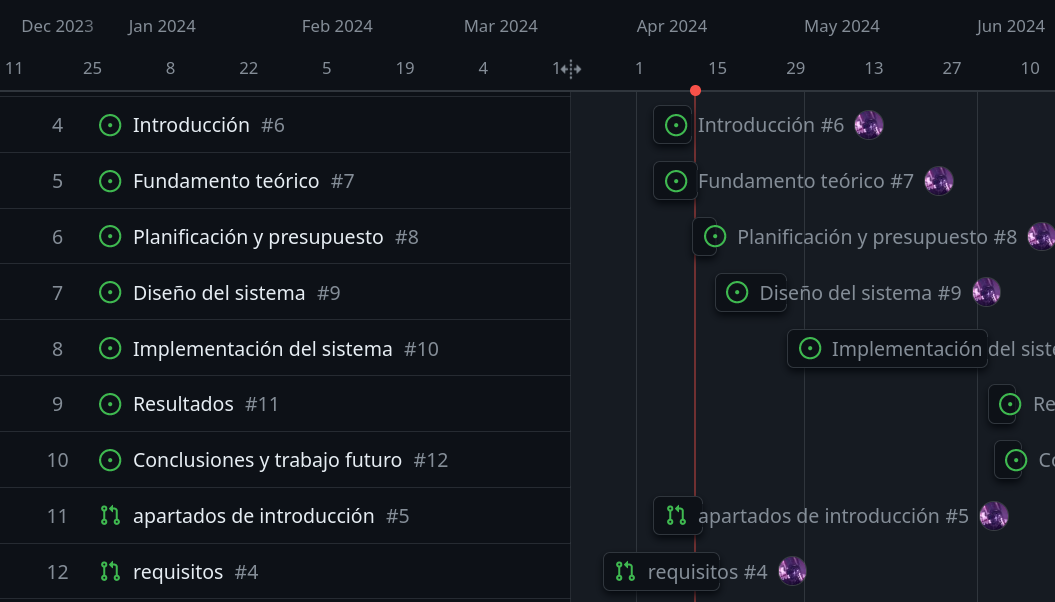
\includegraphics[width=0.9\textwidth]{roadmap.png}
			\captionof{figure}{Roadmap de apartados de la memoria}
		\end{minipage}
\end{itemize}


\subsection{Comunicación}\label{subsec:comunicación}
La comunicación con los tutores y con el equipo de desarrollo se considera fundamental para el
correcto desarrollo del proyecto. Puesto que el trabajo se desarrolla de manera presencial en
la oficina de la empresa, la comunicación con el equipo de desarrollo se realiza de manera
frecuente y directa, mientras que la comunicación con los tutores se realiza de manera remota
pero igual de frecuente, manteniendo el contacto mediante correo electrónico y Teams para
pedir revisiones e informar sobre el estado del trabajo en todo momento.

\subsection{Plataformas de planificación}\label{subsec:plataformas}
Con el objetivo de facilitar las tareas de desarrollo y cumplimentar los requisitos por parte
de la empresa, se utilizan las siguientes plataformas y herramientas de desarrollo para la
fabricación del proyecto:

\begin{itemize}
	\item \textbf{GitHub}: Plataforma de desarrollo colaborativo para el desarrollo del proyecto.
		Se utiliza para la gestión de tareas, seguimiento de desarrollo, documentación y
		colaboración.
	\item \textbf{Atlassian suite (\emph{Jira, Bitbucket})}: Suite de herramientas de gestión de proyectos
		y desarrollo colaborativo. Se utiliza para el desarrollo y documentación del proyecto de
		parte de la empresa.
	\item \textbf{Microsoft Teams}: Herramienta de comunicación y colaboración en tiempo real.
	\item \textbf{Microsoft Outlook}: Herramienta de comunicación por correo electrónico.
\end{itemize}

\newpage{}
\section{Presupuesto}\label{sec:presupuesto}

\chapter{Análisis}\label{chap:analisis}
Este capítulo se centra en desglosar los componentes críticos del proyecto, específicamente
dirigido a entender las necesidades de Okticket y cómo el desarrollo propuesto se alinea con estas.
Se analizarán los requisitos funcionales y no funcionales, evaluando cómo cada uno contribuye al
éxito del proyecto. Además, se identificarán las partes interesadas clave y se explorarán sus
expectativas y requisitos, para asegurar que el sistema desarrollado cumpla con sus necesidades
específicas. Este análisis detallado tiene como objetivo final proporcionar una hoja de ruta
clara para el desarrollo del proyecto, asegurando que se tomen decisiones informadas que maximicen
el valor entregado a la empresa y sus clientes.

\section{Partes interesadas (stakeholders)}\label{sec:stakeholders}
Las partes interesadas en el proyecto son aquellas personas o entidades que tienen un interés
en el mismo, ya sea porque se ven afectadas por el resultado del proyecto, o porque tienen
algún tipo de interés en el mismo. Las partes interesadas en este proyecto son las siguientes:

\begin{enumerate}
	\item \textbf{Okticket}: la empresa es la principal parte interesada en el proyecto, ya que
		es la que se beneficiará directamente de los resultados del mismo, así como de las
		oportunidades de negocio que se abren con la explotación de los datos. Dentro de la empresa,
		se pueden identificar dos entidades:
		\begin{itemize}
			\item \textbf{Equipo de desarrollo de la empresa}: el equipo de desarrollo es otra parte
				interesada en el proyecto, ya que son los encargados de llevar a cabo la implementación
				del sistema y de garantizar su correcto funcionamiento, además de gestionar el soporte
				de servicio a nivel técnico.
			\item \textbf{Equipo de soporte de la empresa}: el sistema planteado ahorraría tiempo al equipo de
				soporte, ya que les permitiría analizar los datos de forma más eficiente e identificar
				problemas antes de que tener que resolver las peticiones de los clientes afectados a
				nivel básico.
		\end{itemize}
	\item \textbf{Clientes}: los clientes de la empresa también son partes interesadas, puesto
		que se beneficiarán de los nuevos servicios que se ofrecen, como los dashboards de
		negocio que se han descrito anteriormente.
	\item \textbf{Investigador y desarrollador (\emph{\author}):} el desarrollador del
		proyecto tiene la oportunidad de aplicar los conocimientos adquiridos en el desarrollo de un
		proyecto real, y de adquirir nuevos conocimientos en el proceso.
\end{enumerate}

\section{Valoración de alternativas}\label{sec:alternativas}


\section{Definición del sistema}\label{sec:definicion}

\input{sections/5_diseño.tex}
\chapter{Implementación}

\chapter{Resultados}

\chapter{Resultados y trabajo futuro}
El propósito de este capítulo es presentar las conclusiones obtenidas a partir
del desarrollo del proyecto, recopilar las dificultades encontradas y proponer
líneas de trabajo futuro en vista a la amplicación y mejora del sistema.

\section{Resultados}
El resultado del proyecto es un sistema de monitorización y análisis de datos
funcional y escalable, que permite a los usuarios obtener insights valiosos a
partir de la información recopilada.

Se ha logrado implementar una arquitectura robusta y flexible, basada en
tecnologías modernas y en la nube, que facilita la ingesta, procesamiento y
visualización de datos de manera eficiente y sencilla.

El sistema es capaz de ingestar datos de diversas fuentes, como bases de datos
internas, logs de aplicaciones y servicios externos, y de presentarlos de forma
clara y útil a través de Kibana.

La infraestructura se despliega y orquesta de manera automática en la nube,
permitiendo una gestión sencilla y eficiente del sistema para los
administradores.

Pese a que no se han completado todas las historias de usuario planificadas,
se han logrado los objetivos principales del proyecto, sentando las bases para
futuras iteraciones y logrando así entregar un producto mínimo viable (MVP).

El motivo de no haber completado todas las historias de usuario planificadas
se debe al tamaño y naturaleza del proyecto, que ha resultado ser más complejo
de lo esperado en un principio. Sin embargo, se ha logrado superar los objetivos
principales y se ha entregado un producto funcional y de calidad.


\newpage{}
\section{Trabajo futuro}
El proyecto ha sentado las bases para un sistema de monitorización y análisis de
datos robusto y escalable. Sin embargo, existen áreas de mejora y ampliación que
podrían ser abordadas en futuras iteraciones.


\subsection{Historias de usuario restantes}
Lo primero de todo sería completar las historias de usuario menos críticas que
han quedado pendientes, como la ingesta de datos de APIs externas o el
\textit{web scraping}. Estas funcionalidades permitirían enriquecer los datos
disponibles y ampliar las fuentes de información.

\begin{table}[H]
	\centering
	\begin{tabular}{|p{0.7\linewidth}|c|c|}
		\hline
		\textbf{Nombre} & \textbf{Prioridad} & \textbf{Tamaño} \\
		\hline
		\hline
		Como desarrollador de Okticket, quiero que los datos contengan metadatos que faciliten su filtrado o búsqueda & P2\cellcolor{yellow!50} & XS\cellcolor{blue!25} \\
		\hline
		Como trabajador de Okticket, quiero poder ver y consultar datos de empresas cliente & P2\cellcolor{yellow!50} & S\cellcolor{green!25} \\
		\hline
		Como gestor de una empresa cliente, quiero poder ver información relevante sobre mi empresa que recoja Okticket & P2\cellcolor{yellow!50} & M\cellcolor{yellow!50} \\
		\hline
		Como desarrollador de Okticket, quiero poder ingestar datos de APIs externas a la empresa & P2\cellcolor{yellow!50} & M\cellcolor{yellow!50} \\
		\hline
		Como desarrollador de Okticket, quiero poder ingestar información de páginas web externas (\textit{scraping}) & P2\cellcolor{yellow!50} & S\cellcolor{green!25} \\
		\hline
	\end{tabular}
	\caption{Historias de usuario restantes para futuras iteraciones}
	\label{tab:remaining_tasks}
\end{table}

Como se puede observar en la tabla \ref{tab:remaining_tasks}, las historias de
usuario restantes son las menos prioritarias (siguiendo con
\fullref{sec:planif_inicial}).

\newpage{}
\subsection{Integración de lenguaje natural para búsqueda (DSL)}
Sería interesante explorar la posibilidad de integrar el sistema con
un sistema de búsqueda y filtrado de datos a través de lenguaje natural, como
\textit{Natural Language Processing} (NLP)\footnote{
	\url{https://www.elastic.co/guide/en/elasticsearch/reference/current/query-dsl-query-string-query.html}
}

Esto permitiría a los usuarios realizar consultas de manera más intuitiva y
eficiente, sin necesidad de conocer la sintaxis de Kibana Query Language (KQL).


\subsection{Aplicación de modelos de Lenguaje de Gran Escala (LLM)}
Desde la empresa, se ha propuesto la posibilidad de aplicar modelos de LLM
para la generación de texto automática, presumiblemente de manera agnóstica al
proveedor (OpenAI, Anthropic, Google\ldots).

Esto permitiría la generación de informes y análisis de manera automática a
partir de los datos recopilados, facilitando la toma de decisiones y la
comunicación de insights a los usuarios.

\subsection{Más perspectivas futuras}
Gracias a la flexibilidad del stack ELK, se podrían añadir nuevas fuentes de
datos y visualizaciones, como logs de otras partes de la aplicación (gestor web,
otros servicios internos como Hubspot o Holded, aplicación móvil\ldots) o
visualizaciones más avanzadas y personalizadas.

Lo bueno de haber diseñado la arquitectura de la manera que se ha hecho
es que se pueden añadir nuevas funcionalidades sin necesidad de modificar
la infraestructura existente, simplemente añadiendo nuevos servicios y
configuraciones.

La escalabilidad del sistema también es un punto a tener en cuenta. En caso de
necesitar más capacidad de procesamiento o almacenamiento, se podría establecer
un sistema de autoescalabilidad en base a las definiciones ya realizadas.

Por último, se podría explotar la funcionalidad del stack de generar alertas
en base a la información ingestada y procesada, para notificar a los usuarios
de eventos críticos o anomalías detectadas en los datos.


\newpage{}
\section{Conclusiones y retrospectiva}
El desarrollo de este proyecto me ha permitido, a nivel personal, adquirir
conocimientos y habilidades muy útiles en áreas que tienen una gran demanda en
el mercado laboral actual, como la ingesta y procesamiento de datos, la
orquestación de servicios en la nube y la experiencia con proveedores cloud como
AWS.

A nivel técnico, he aprendido a trabajar con tecnologías modernas y potentes,
como Kafka, Logstash, Elasticsearch y Kibana, que me han permitido implementar
una solución robusta y escalable para la monitorización y análisis de datos.

Además, he tenido la oportunidad de trabajar con metodologías ágiles y de
gestión de proyectos, como Scrum, en proyectos reales con repercusiones y
resultados tangibles.

En cuanto a la retrospectiva del proyecto, considero que el tiempo dedicado ha
merecido la pena, pero podría haber sido gestionado u organizado diferente.


%% Esto incluirá la bibliografía correctamente en nuestro trabajo
\newpage % En una nueva página
\addcontentsline{toc}{chapter}{Bibliografía} % Añade la referencia al índice de contenido

\bibliographystyle{ieeetr} % Define el estilo de la bibliografía
\bibliography{biblio} % Indica el archivo que contiene la colección de citas

\nocite{template}
\nocite{mier2024anomalias}

\end{document}
